\chapter{平稳作用量与欧拉--拉格朗日方程}

\lectureoverview{人们熟悉的名称\emph{最小作用量原理}掩盖了要点：物理轨迹使作用量平稳，但不必使其取极小值。我们将从普通的平衡出发建立这一陈述，把它从点推广到整个函数，通过离散化一条路径推导出欧拉--拉格朗日方程，并重新得到牛顿方程。旋转坐标和极坐标随后将表明，为什么拉格朗日表述不仅仅是一种记号上的改变。}

\section{平稳，而不必取极小}

传统名称中不可靠的部分是\emph{最小}一词。经典轨迹并不总是使作用量取极小值。它也可能在可能轨迹的空间中给出极大值或鞍点。正确的原理是作用量\emph{平稳}：它的一阶变化为零。

从较简单的平衡问题开始。保持静止的粒子没有加速度，因此其净力必须为零。对于由一维势导出的力，
\begin{equation}
  F(x)=-\frac{dV}{dx},
  \label{eq:force-from-v}
\end{equation}
平衡条件为
\begin{equation}
  \frac{dV}{dx}=0.
  \label{eq:stationary-v-one}
\end{equation}

\begin{figure}[htbp]
  \centering
  \includegraphics[width=0.74\textwidth]{lecture_03_figure_02.png}
  \caption{一维平衡条件：力在势平稳处为零。}
  \lectureframe{00:02:51}
\end{figure}

现在把粒子移动一个小量\(\delta x\)。到一阶，
\begin{equation}
  \delta V
  =V(x+\delta x)-V(x)
  =\frac{dV}{dx}\,\delta x+O(\delta x^2).
  \label{eq:first-variation-one}
\end{equation}
在平衡处，无论\(\delta x\)的符号如何，线性项都为零：
\begin{equation}
  \delta V=0
  \qquad\hbox{to first order.}
  \label{eq:delta-v-zero-one}
\end{equation}
这并不意味着在有限移动之后\(V\)完全不变。它说的是，主导变化是二阶或更高阶的。极小值和极大值都满足这一条件。

\begin{figure}[htbp]
  \centering
  \begin{tikzpicture}[scale=0.95,>=Latex]
    \draw[->] (-0.2,0) -- (3.35,0) node[right] {$x$};
    \draw[->] (0,-0.2) -- (0,2.25) node[above] {$V$};
    \draw[blue!65!black,thick,smooth]
      plot coordinates {(0.2,1.85) (0.75,0.85) (1.55,0.35)
                        (2.35,0.85) (3.0,1.85)};
    \fill[red!65!black] (1.55,0.35) circle (2pt);
    \node at (1.55,-0.34) {minimum};
    \begin{scope}[xshift=4.25cm]
      \draw[->] (-0.2,0) -- (3.35,0) node[right] {$x$};
      \draw[->] (0,-0.2) -- (0,2.25) node[above] {$V$};
      \draw[blue!65!black,thick,smooth]
        plot coordinates {(0.2,0.35) (0.75,1.25) (1.55,1.85)
                          (2.35,1.25) (3.0,0.35)};
      \fill[red!65!black] (1.55,1.85) circle (2pt);
      \node at (1.55,-0.34) {maximum};
    \end{scope}
  \end{tikzpicture}
  \caption{平稳性确定一阶导数，而不确定该点是极小值还是极大值。}
  \label{fig:min-max-stationary}
\end{figure}

对于多个坐标\(q_i\)，一阶变分为
\begin{equation}
  \delta V
  =\sum_i\frac{\partial V}{\partial q_i}\,\delta q_i.
  \label{eq:first-variation-many}
\end{equation}
如果这对每一个独立的无穷小位移\(\delta q_i\)都必须为零，那么每个系数都为零：
\begin{equation}
  \frac{\partial V}{\partial q_i}=0
  \qquad\hbox{for every }i.
  \label{eq:stationary-v-many}
\end{equation}

二维势最好想象成起伏的地形，而不是过山车。平稳点可能是谷底、山顶或鞍点。在鞍点处，沿一个方向的运动起初上升，而沿另一个方向的运动起初下降。因此，恢复行为可以在一个方向上稳定，而在另一个方向上不稳定，尽管在点本身处所有一阶导数都为零。

\begin{figure}[htbp]
  \centering
  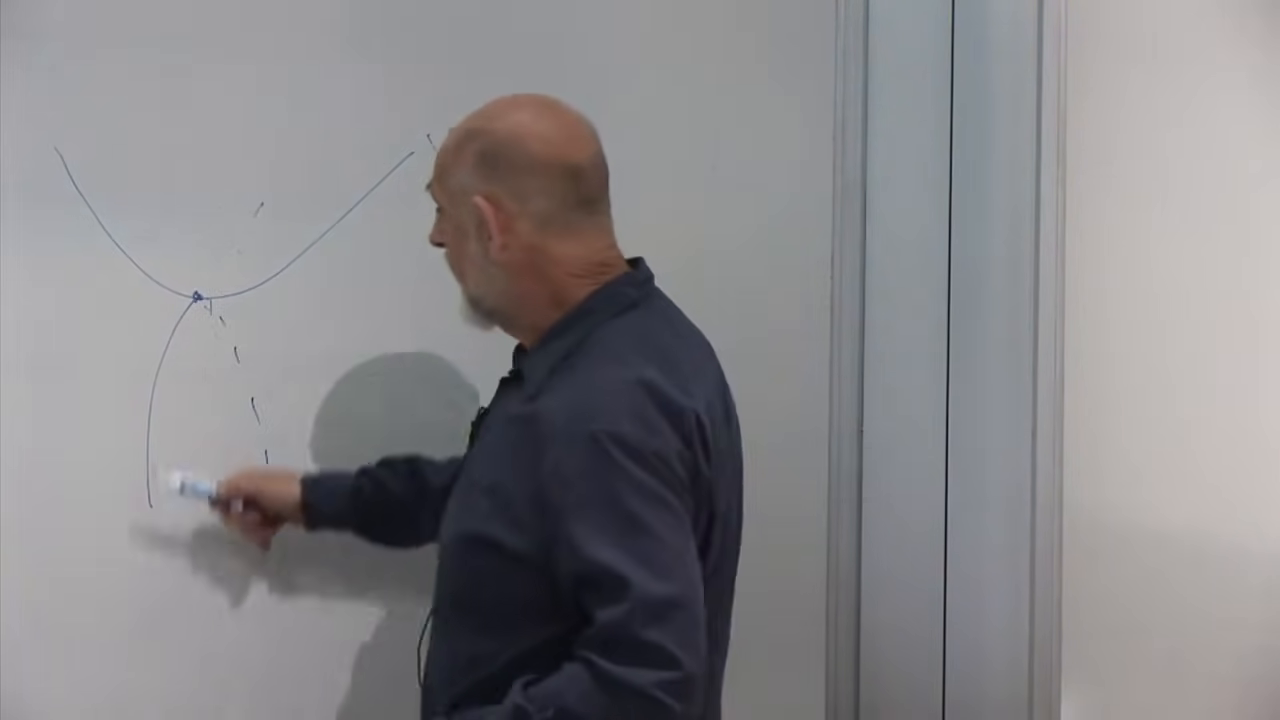
\includegraphics[width=0.76\textwidth]{lecture_03_figure_06.png}
  \caption{鞍点在每个一阶方向上都是平稳的，尽管相邻位移沿一个轴上升，沿另一个轴下降。}
  \lectureframe{00:08:20}
\end{figure}

在具有许多坐标的空间中，鞍点比纯粹的极大值或极小值更典型。这就是为什么\emph{平稳}是更持久的词。条件
\begin{equation}
  \delta V=0
  \label{eq:equilibrium-variation}
\end{equation}
概括了平衡，而不预先判断二阶行为。

\section{从点到函数}

力学关注的是整个运动，而不是孤立的平衡点。轨迹是一个函数，例如\(x(t)\)，或一个集合\((x(t),y(t),z(t))\)。通过变分整个函数使某个量平稳的数学问题就是\emph{变分法}。在把它应用于运动之前，先考虑三个较简单的例子。

\subsection{最短曲线与测地线}

在平面中固定两个点，并用\(y(x)\)表示它们之间的一条曲线。在一小段上，
\begin{equation}
  ds=\sqrt{dx^2+dy^2}
  =dx\sqrt{1+\left(\frac{dy}{dx}\right)^2},
  \label{eq:line-element}
\end{equation}
其中最后一种形式假设\(dx>0\)。总长度为泛函
\begin{equation}
  S[y]=\int_{x_0}^{x_1}
  \sqrt{1+y'(x)^2}\,dx.
  \label{eq:arc-length-functional}
\end{equation}
方括号强调\(S\)以整个函数为输入。直线由
\begin{equation}
  \delta S=0
  \label{eq:stationary-length}
\end{equation}
在保持两个端点固定的曲线小变化下选出。

\begin{figure}[htbp]
  \centering
  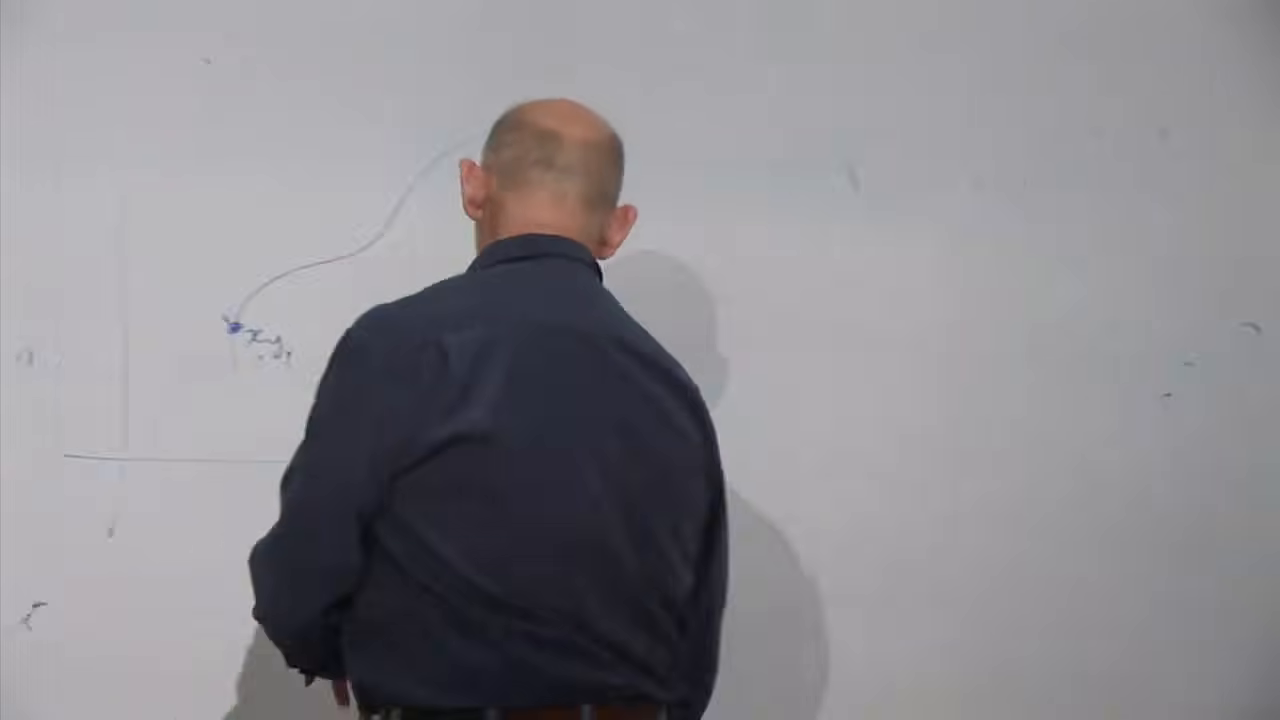
\includegraphics[width=0.78\textwidth]{lecture_03_figure_07.png}
  \caption{两个固定端点之间的一条试探曲线。其长度是无穷小斜边\(ds\)之和。}
  \lectureframe{00:13:36}
\end{figure}

同样的问题可以在曲面上提出。在两个桩之间拉紧一根绳子，给出了最短受约束路径的物理图像。这样一条长度为平稳值的曲线就是\emph{测地线}。在平面上它是直线；在球面或起伏曲面上，它一般不是直线。

\subsection{费马原理}

在速度随位置变化的介质中，光线\(c(x,y)\)不必沿最短的空间路径传播。一小段所需的时间是距离除以局部速度，因此
\begin{equation}
  T[y]
  =\int_{x_0}^{x_1}
  \frac{\sqrt{1+y'(x)^2}}{c(x,y)}\,dx.
  \label{eq:fermat-functional}
\end{equation}
费马原理要求
\begin{equation}
  \delta T=0.
  \label{eq:fermat-stationary}
\end{equation}
当\(c\)为常数时，这归结为最短距离问题。然而，在折射率变化的介质中，最快的路径要在距离与局部传播速度之间取得平衡。

\begin{figure}[htbp]
  \centering
  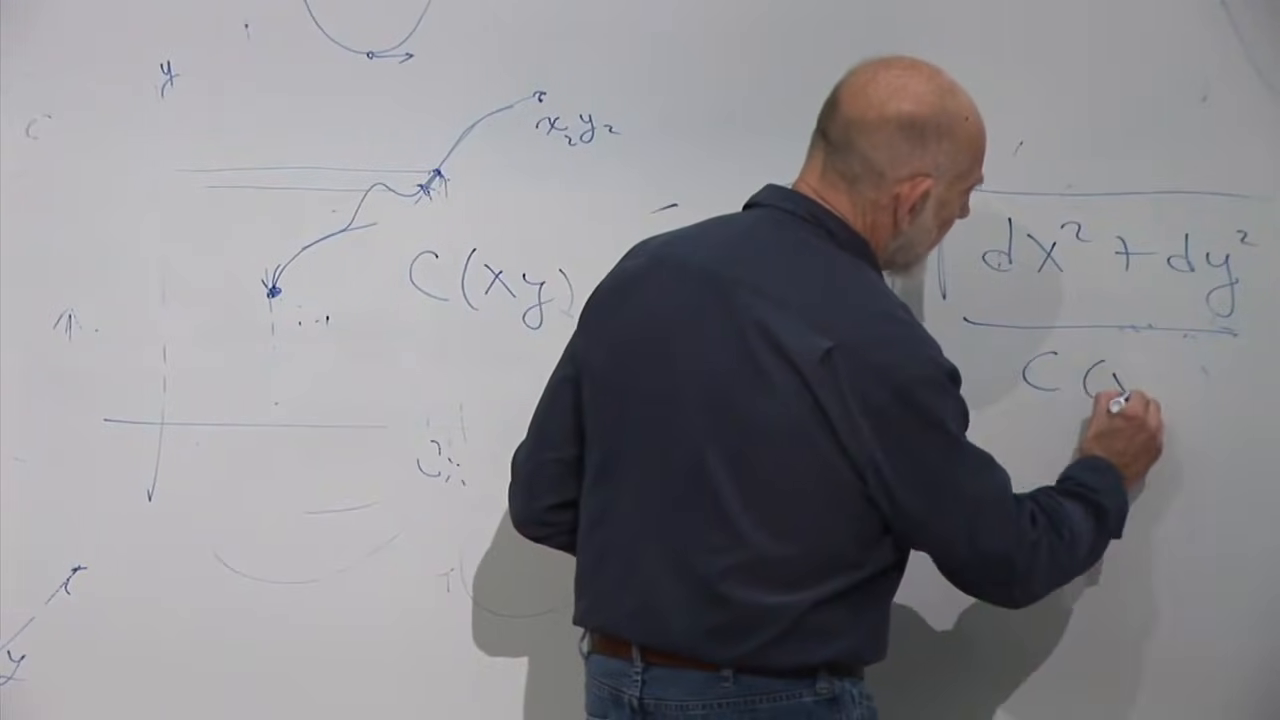
\includegraphics[width=0.80\textwidth]{lecture_03_figure_08.png}
  \caption{光线在局部光速依赖于位置的介质中的最短时间泛函。}
  \lectureframe{00:22:50}
\end{figure}

一个应景的笑话提到了当时新近的说法：中微子在意大利以异常快的速度运动。物理学的论证随即回到可靠的例子：普通光在材料中根据折射率改变速率。

\subsection{悬挂的链条}

两端固定的链条会稳定成悬链线。每一小段都贡献引力势能，因此总势能本身就是沿链条的积分。端点再次固定，未知形状是一个函数，而某个积分必须取驻值。

\begin{figure}[htbp]
  \centering
  \includegraphics[width=0.76\textwidth]{lecture_03_figure_03.png}
  \caption{固定支座之间的悬挂链条。其驻定形状由总引力势能选定。}
  \lectureframe{00:30:41}
\end{figure}

这些例子具有相同的架构：两个固定端点、它们之间的一个函数，以及一个其一阶变分为零的积分。把这样一种整体指令化为微分方程，正是求解变分问题的含义。

\section{作为边值问题的力学}

轨迹常被画成时间水平，因为 \(t\) 是自变量。然而物理学中有一个很强的惯例，把时间画成竖直向上。一段题外话回顾了这样的实验：人们按照与自身书写系统相关的方向，把照片从年轻到年老排列；从左到右阅读的人倾向于从左到右排列，从右到左阅读的人则相反，而受过纵向阅读训练的人则纵向排列。笑话的结论是，物理学家就是坚持时间向上流动的人。这里我们将使用传统的水平 \(t\) 轴，因为它使 \(x(t)\) 读起来自然地像一幅图。

在初值表述中，\(t_0\) 处的数据是
\begin{equation}
  x(t_0)=x_0,
  \qquad
  \dot x(t_0)=v_0.
  \label{eq:initial-value-data}
\end{equation}
牛顿方程随后决定其后的轨道。变分表述提出的是另一个问题：指定两个端点事件，
\begin{equation}
  x(t_0)=x_0,
  \qquad
  x(t_1)=x_1,
  \label{eq:boundary-value-data}
\end{equation}
并确定它们之间的物理路径。初速度不再被给定；它成为解的一部分。

\begin{figure}[htbp]
  \centering
  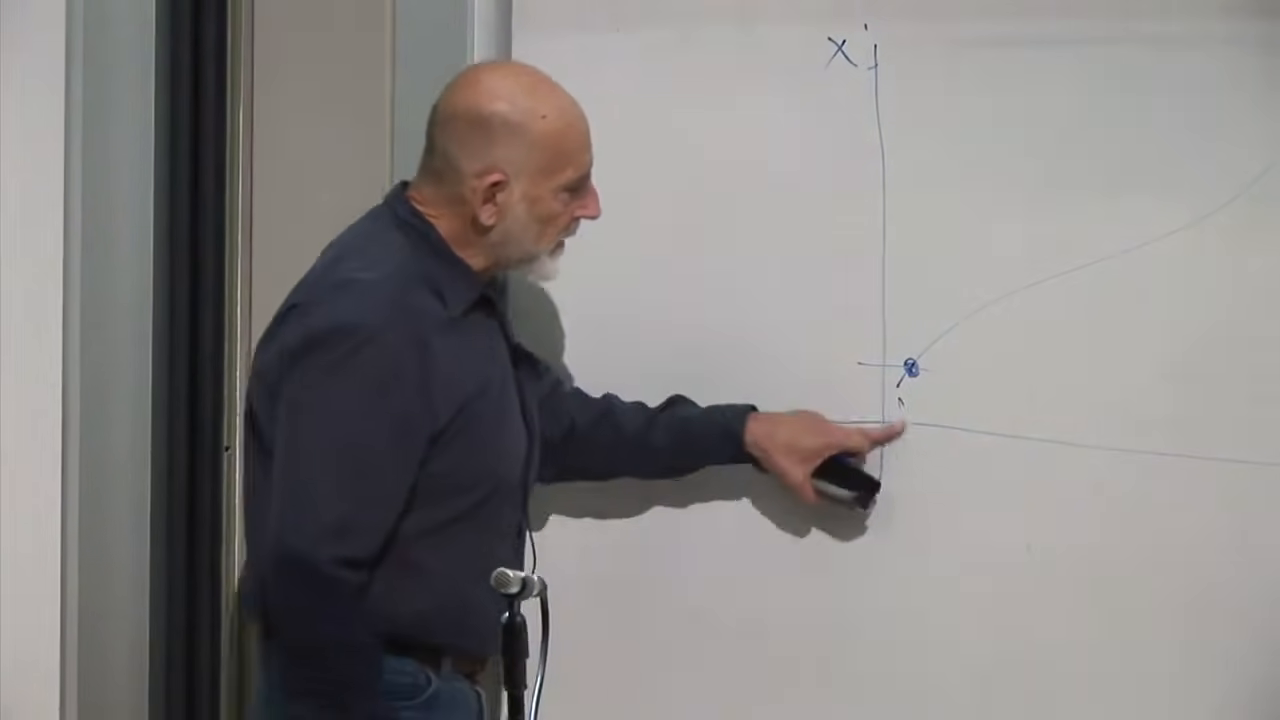
\includegraphics[width=0.76\textwidth]{lecture_03_figure_09.png}
  \caption{一条力学轨迹 \(x(t)\)。可以在一端指定位置和斜率，或在两个端点时刻指定位置。}
  \lectureframe{00:27:41}
\end{figure}

要被取为驻值的量是 \emph{作用量}，
\begin{equation}
  A[x]=\int_{t_0}^{t_1}L(x,\dot x,t)\,dt.
  \label{eq:action-one}
\end{equation}
被积函数 \(L\) 是 \emph{拉格朗日量}。它可能依赖于位置、速度，并显式依赖于时间。作用量原理是
\begin{equation}
  \delta A=0
  \label{eq:stationary-action}
\end{equation}
对所有满足
\begin{equation}
  \delta x(t_0)=\delta x(t_1)=0.
  \label{eq:fixed-endpoint-variations}
\end{equation}
的小路径变分成成立。端点条件至关重要：我们比较的是连接同样两个事件的邻近路径。

\section{欧拉--拉格朗日方程的离散推导}

作用量是无穷多个路径值的泛函。为了使它的变分具体化，把时间区间分成若干长度为\(\epsilon\)的步长，
\begin{equation}
  t_n=t_0+n\epsilon,
  \qquad
  x_n=x(t_n),
  \label{eq:discrete-times}
\end{equation}
并将第\(n\)个区间上的速度近似为
\begin{equation}
  v_n=\frac{x_{n+1}-x_n}{\epsilon}.
  \label{eq:discrete-velocity}
\end{equation}
该积分变为普通求和
\begin{equation}
  A_\epsilon
  =\sum_{n=0}^{N-1}
  \epsilon L\left(x_n,\frac{x_{n+1}-x_n}{\epsilon}\right).
  \label{eq:discrete-action}
\end{equation}
我们用\(n\)作为时间切片的标号，以便\(i\)留待后面用于空间坐标和粒子。

\begin{figure}[htbp]
  \centering
  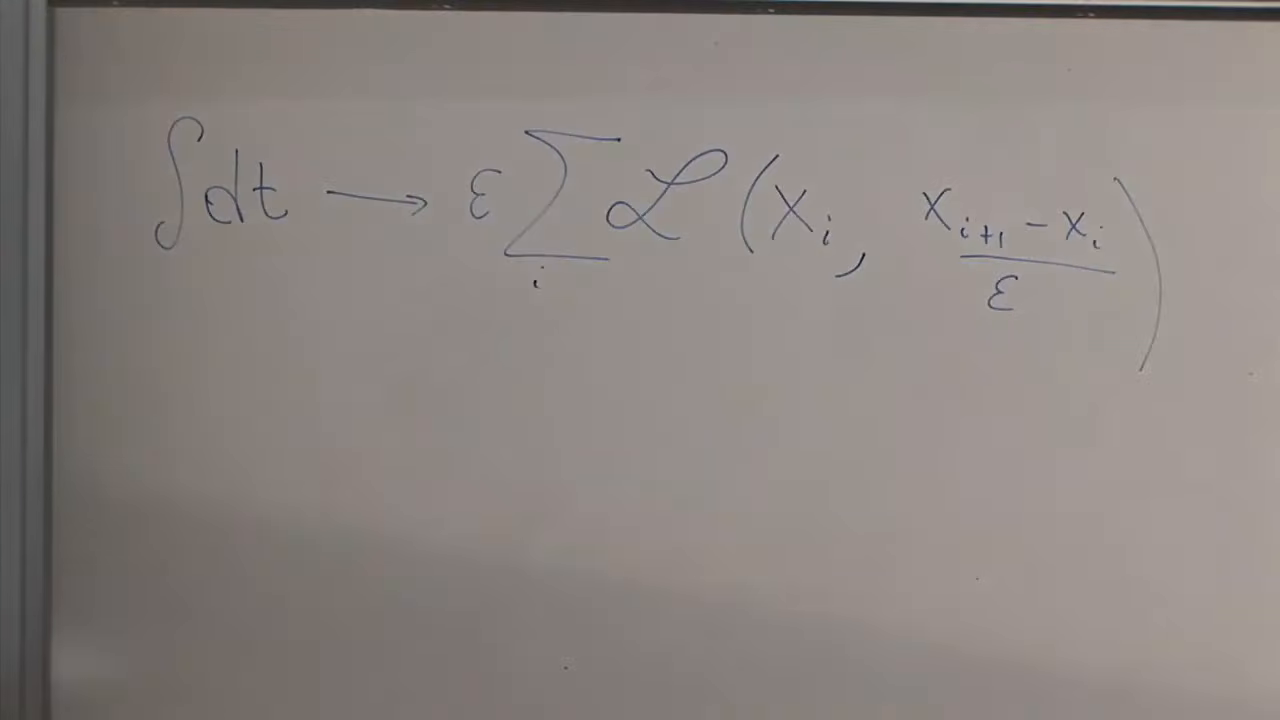
\includegraphics[width=0.82\textwidth]{lecture_03_figure_10.png}
  \caption{轨迹被替换为一串时间切片。改变一个内部高度只会改变其相邻的两段。}
  \lectureframe{00:38:30}
\end{figure}

改变一个内部点 \(x_n\)，保持所有其他 \(x_k\) 固定。求和中只有两项依赖于 \(x_n\)：
\begin{align}
  A_\epsilon\big|_{x_n}
  &=
  \epsilon L\left(x_n,\frac{x_{n+1}-x_n}{\epsilon}\right)
  \notag\\
  &\quad+
  \epsilon L\left(x_{n-1},
                  \frac{x_n-x_{n-1}}{\epsilon}\right).
  \label{eq:two-neighbor-terms}
\end{align}
求导给出
\begin{align}
  0=\frac{\partial A_\epsilon}{\partial x_n}
  &=
  \epsilon\frac{\partial L_n}{\partial x_n}
  -\frac{\partial L_n}{\partial v_n}
  +\frac{\partial L_{n-1}}{\partial v_{n-1}}.
  \label{eq:discrete-el-variation}
\end{align}
相反的符号有一个简单的几何来源。提高 \(x_n\) 会增大它后面区间的斜率，并减小它前面区间的斜率。

\begin{figure}[htbp]
  \centering
  \includegraphics[width=0.74\textwidth]{lecture_03_figure_04.png}
  \caption{离散变分中直接的位置导数与两个相邻的速度导数贡献。}
  \lectureframe{00:45:26}
\end{figure}

重排式~\eqref{eq:discrete-el-variation}：
\begin{equation}
  \frac{1}{\epsilon}
  \left(
    \frac{\partial L_n}{\partial v_n}
    -\frac{\partial L_{n-1}}{\partial v_{n-1}}
  \right)
  =
  \frac{\partial L_n}{\partial x_n}.
  \label{eq:discrete-el}
\end{equation}
左边是一个相邻差商。当
\(\epsilon\to0\) 时，折线变成光滑路径，而该商变成时间导数：
\begin{equation}
  \boxed{
  \frac{d}{dt}\left(\frac{\partial L}{\partial\dot x}\right)
  =
  \frac{\partial L}{\partial x}}
  .
  \label{eq:euler-lagrange-one}
\end{equation}
这就是欧拉--拉格朗日方程。

\begin{figure}[htbp]
  \centering
  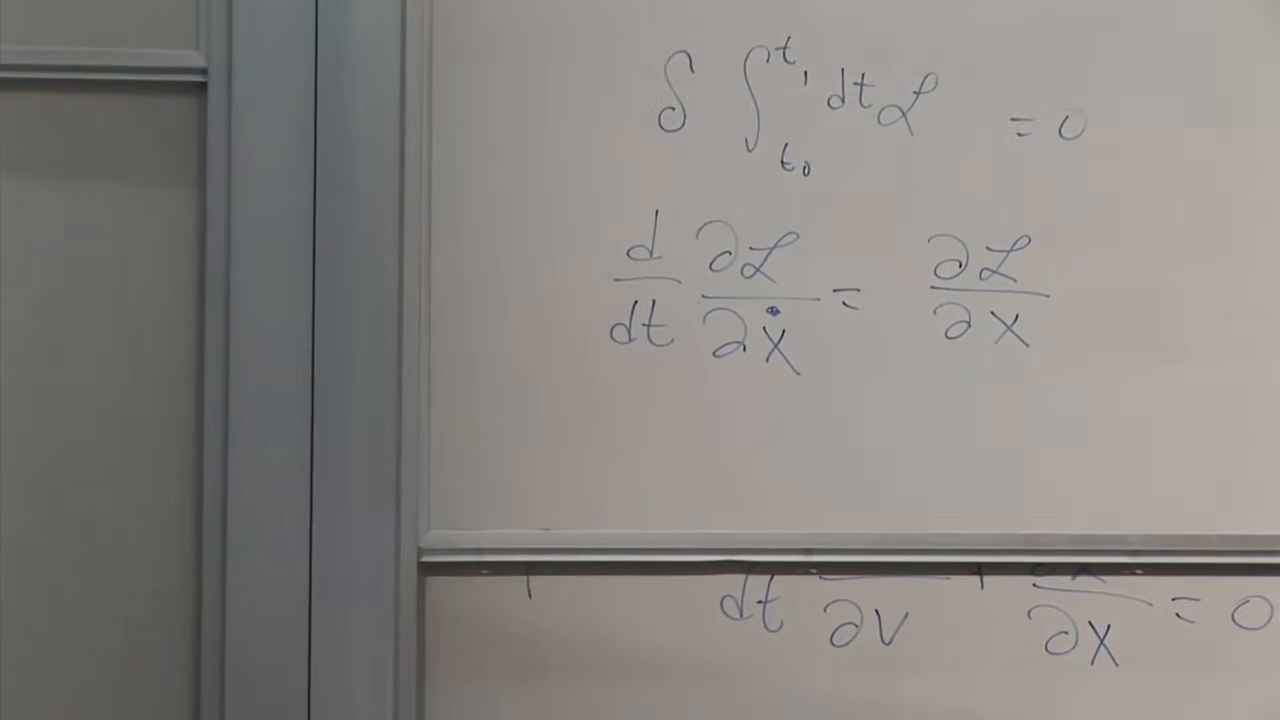
\includegraphics[width=0.78\textwidth]{lecture_03_figure_11.png}
  \caption{由每个内部时间切片处的驻定性得到的完整欧拉--拉格朗日方程。}
  \lectureframe{00:49:25}
\end{figure}

一旦指定了 \(L\)，式~\eqref{eq:euler-lagrange-one} 就充当一台机器：对给定函数求导，机器便返回路径所满足的微分方程。

\begin{classroomqa}
  \audiencequestion{欧拉--拉格朗日结果对\(x\)和\(\dot x\)的任意函数都成立吗？\lecturetimestamp{00:49:37--00:50:24}}
  \lecturerresponse{是的，前提是导数所需的正则性得到满足。
  弧长例子在将其自变量\(x\)重新标记为\(t\)所扮演的角色、并将其未知函数\(y(x)\)重新标记为\(x(t)\)所扮演的角色之后，具有完全相同的形式。其欧拉--拉格朗日方程具有直线解。}
\end{classroomqa}

\section{从拉格朗日量得到牛顿方程}

对于势\(V(x)\)中直线上的一个粒子，取
\begin{equation}
  L(x,\dot x)=T-V
  =\frac12m\dot x^2-V(x).
  \label{eq:lagrangian-tv-one}
\end{equation}
负号可能看起来奇怪，因为总能量是\(T+V\)。但拉格朗日量不是能量。它的检验标准是欧拉--拉格朗日机器是否返回正确的运动。关于符号的模拟投票被拒绝：答案必须被检验，而不是被选举。

首先，
\begin{equation}
  \frac{\partial L}{\partial\dot x}=m\dot x.
  \label{eq:conjugate-momentum-one}
\end{equation}
这就是动量。更一般地，与任意坐标\(q\)共轭的动量定义为
\begin{equation}
  p_q=\frac{\partial L}{\partial\dot q}.
  \label{eq:conjugate-momentum-general}
\end{equation}
对式~\eqref{eq:conjugate-momentum-one}取时间导数得到
\(m\ddot x\)，而
\begin{equation}
  \frac{\partial L}{\partial x}
  =-\frac{dV}{dx}.
  \label{eq:lagrangian-position-derivative}
\end{equation}
因此欧拉--拉格朗日方程是
\begin{equation}
  m\ddot x=-\frac{dV}{dx}=F(x),
  \label{eq:newton-from-action}
\end{equation}
这就是牛顿第二定律。

\begin{figure}[htbp]
  \centering
  \includegraphics[width=0.80\textwidth]{lecture_03_figure_05.png}
  \caption{动能、势能、\(L=T-V\)，以及恢复出的牛顿方程分量形式，都在同一块黑板上。}
  \lectureframe{00:57:52}
\end{figure}

对于多个坐标\(q_i\)，
\begin{equation}
  L(\mathbf q,\dot{\mathbf q})
  =\sum_i\frac12m_i\dot q_i^{\,2}-V(q_1,q_2,\ldots),
  \label{eq:lagrangian-tv-many}
\end{equation}
并且每个坐标都有一个方程：
\begin{equation}
  \frac{d}{dt}\left(\frac{\partial L}{\partial\dot q_i}\right)
  =\frac{\partial L}{\partial q_i}
  \quad\Longrightarrow\quad
  m_i\ddot q_i=-\frac{\partial V}{\partial q_i}=F_i.
  \label{eq:euler-lagrange-many}
\end{equation}
轨迹仍然是一条曲线，只不过现在穿过高维位形空间。

\begin{classroomqa}
  \audiencequestion{我们是否只是从牛顿定律倒推，并构造出一个能重现答案的泛函？\lecturetimestamp{00:58:07--01:00:04}}
  \lecturerresponse{这不是有成效的观点。拉格朗日量是物理系统的紧凑规格：一个关于所有坐标和速度的函数，把所有运动方程打包在一起。在新理论中，物理学家通常提出作用量并推导方程，而不是分别猜测每一个方程。}
\end{classroomqa}

这种打包是一个优点。坐标自由是另一个优点。直线最短这一陈述并不取决于平面是用笛卡儿坐标、极坐标还是曲线坐标描述的。同样，作用量的驻定性不依赖于坐标，尽管\(L\)的公式以及由此得到的分量方程会改变。

\section{从旋转木马上看自由粒子}

设\((x,y)\)为惯性笛卡儿坐标，并设\((X,Y)\)以角速度\(\omega\)匀速旋转。按照这里使用的取向，
\begin{align}
  x&=X\cos\omega t+Y\sin\omega t,
  \notag\\
  y&=-X\sin\omega t+Y\cos\omega t.
  \label{eq:rotating-coordinate-map}
\end{align}
两坐标系之间的夹角是\(\omega t\)。

\begin{figure}[htbp]
  \centering
  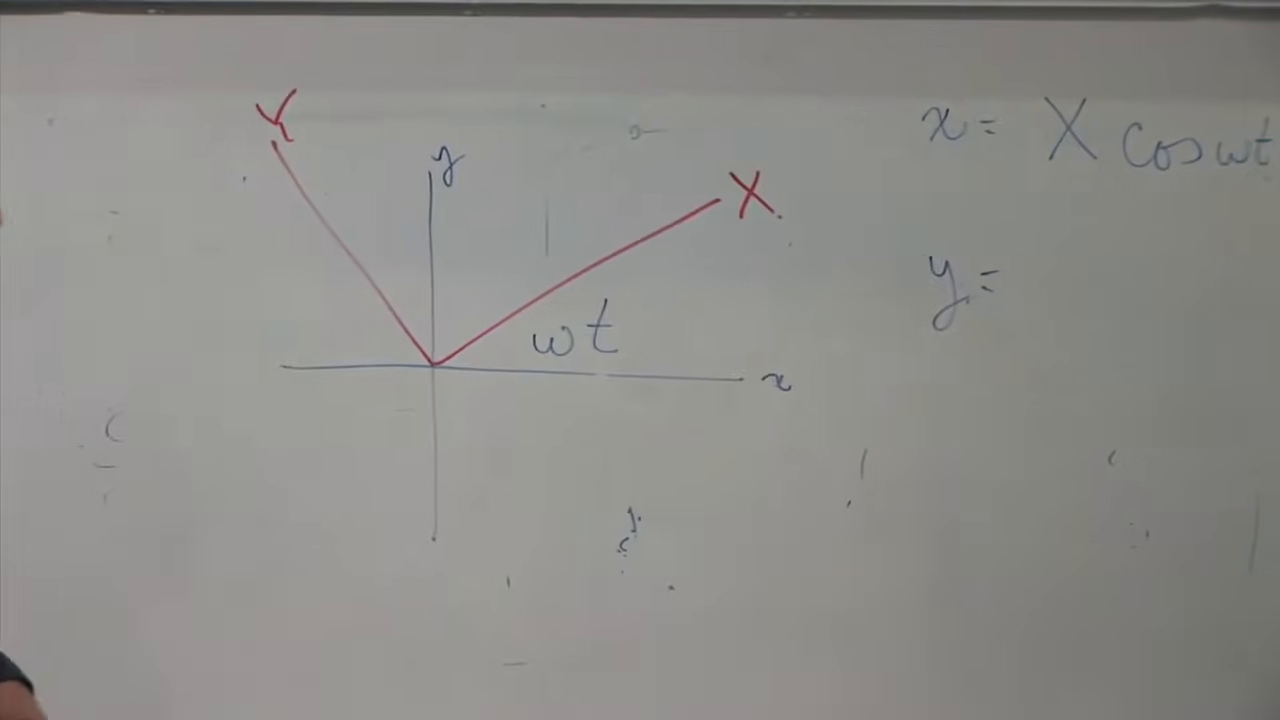
\includegraphics[width=0.76\textwidth]{lecture_03_figure_12.png}
  \caption{惯性笛卡儿轴与匀速旋转笛卡儿轴。同一个点获得依赖于时间的旋转坐标。}
  \lectureframe{01:06:05}
\end{figure}

自由粒子在惯性系中的拉格朗日量为
\begin{equation}
  L_{\mathrm{in}}
  =\frac{m}{2}\left(\dot x^2+\dot y^2\right).
  \label{eq:free-inertial-lagrangian}
\end{equation}
对式~\eqref{eq:rotating-coordinate-map}求导，并使用
\(\sin^2\omega t+\cos^2\omega t=1\)。三角项合并后给出
\begin{align}
  \dot x^2+\dot y^2
  &=
  \dot X^2+\dot Y^2\\
  &\quad+\omega^2(X^2+Y^2)\\
  &\quad+2\omega(Y\dot X-X\dot Y).
  \label{eq:rotating-speed}
\end{align}
因此
\begin{align}
  L_{\mathrm{rot}}
  &=
  \frac{m}{2}(\dot X^2+\dot Y^2)\\
  &\quad+\frac{m\omega^2}{2}(X^2+Y^2)\\
  &\quad+m\omega(Y\dot X-X\dot Y).
  \label{eq:rotating-lagrangian}
\end{align}

\begin{figure}[htbp]
  \centering
  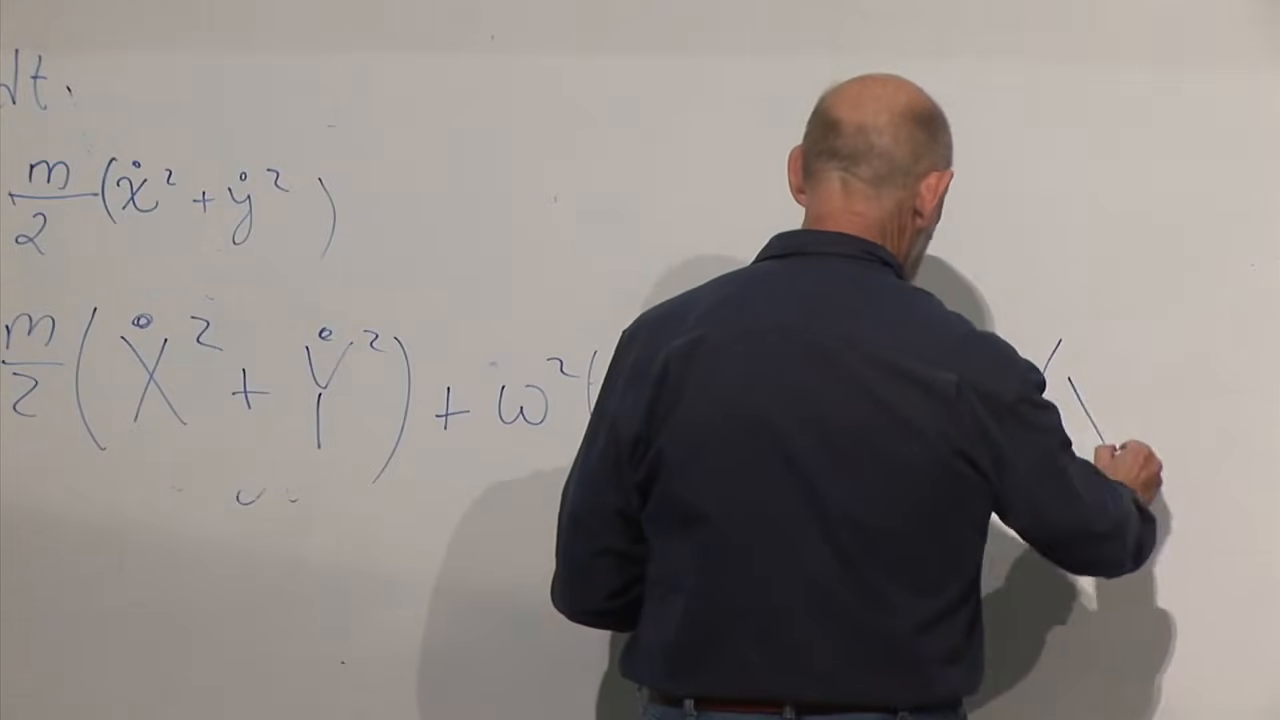
\includegraphics[width=0.84\textwidth]{lecture_03_figure_13.png}
  \caption{变换后的自由粒子拉格朗日量：普通动能、二次离心项，以及一个关于速度线性的项。}
  \lectureframe{01:12:16}
\end{figure}

二次坐标项具有\(-V_{\mathrm{fict}}\)的形式，其中
\begin{equation}
  V_{\mathrm{fict}}
  =-\frac{m\omega^2}{2}(X^2+Y^2).
  \label{eq:centrifugal-potential}
\end{equation}
它向外减小，因此产生离心力
\(m\omega^2(X,Y)\)。

式~\eqref{eq:rotating-lagrangian}中的最后一项对坐标和速度都是线性的。应用欧拉--拉格朗日方程给出
\begin{align}
  m\ddot X&=m\omega^2X-2m\omega\dot Y,
  \notag\\
  m\ddot Y&=m\omega^2Y+2m\omega\dot X.
  \label{eq:rotating-equations}
\end{align}
正比于\(\omega^2\)的项是离心项；正比于速度的项是科里奥利项。在旋转平面内的矢量形式中，
\begin{equation}
  \mathbf F_{\mathrm{C}}
  =-2m\,\boldsymbol\omega\times\mathbf v_{\mathrm{rot}},
  \label{eq:coriolis-vector}
\end{equation}
如果选择相反的取向约定，则符号需要调整。

\begin{figure}[htbp]
  \centering
  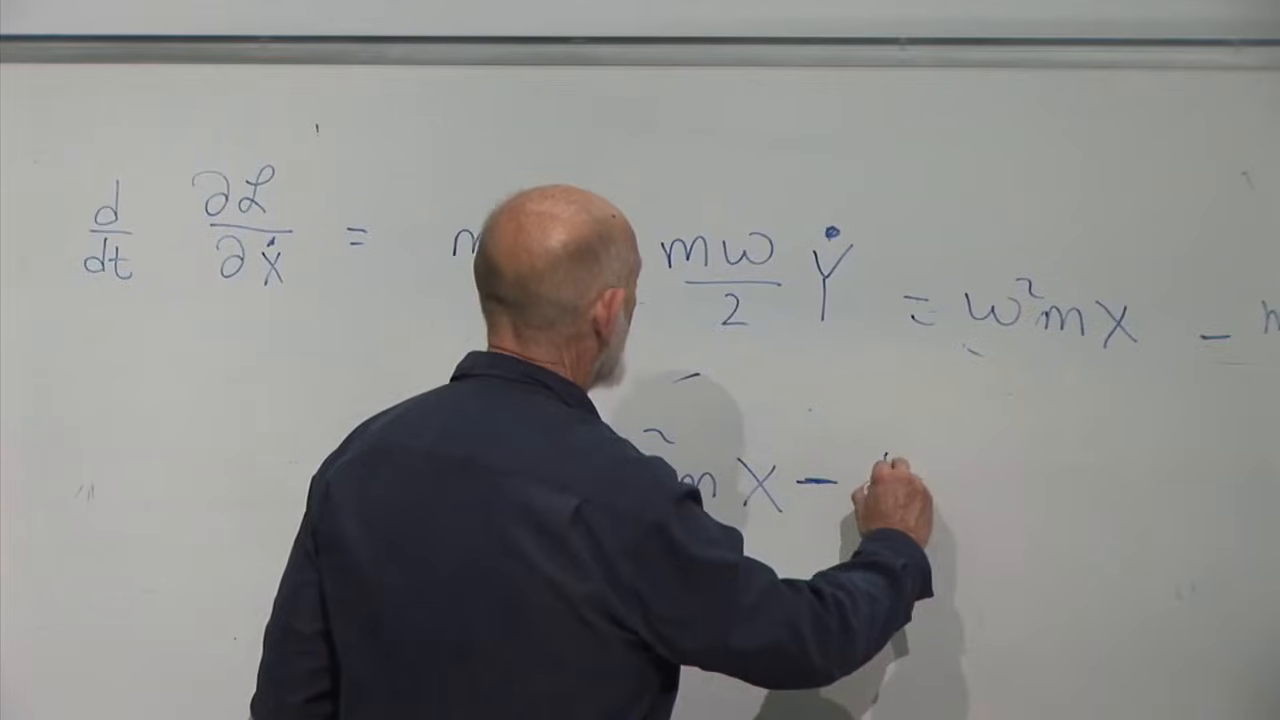
\includegraphics[width=0.84\textwidth]{lecture_03_figure_14.png}
  \caption{旋转系方程，其中正比于坐标的项给出离心加速度，而交叉速度项给出科里奥利加速度。}
  \lectureframe{01:20:20}
\end{figure}

重点不是代数消失了。重点是对一个标量函数作一次坐标变换，就同时生成两个耦合方程和两个虚拟力。

\begin{classroomqa}
  \audiencequestion{这个方法对任意弯曲坐标也有效吗？\lecturetimestamp{01:22:01--01:22:17}}
  \lecturerresponse{是的。新坐标可以是曲线坐标，甚至可以像旋转坐标那样显式依赖于时间。把作用量用新变量重写，并应用同样的欧拉--拉格朗日规则。}
\end{classroomqa}

\section{极坐标与循环角}

对于通常的极坐标，
\begin{equation}
  x=r\cos\theta,
  \qquad
  y=r\sin\theta.
  \label{eq:polar-map}
\end{equation}
\(r\) 和 \(\theta\) 都可以随时间变化。求导并相加平方项，得到
\begin{equation}
  \dot x^2+\dot y^2
  =\dot r^2+r^2\dot\theta^2.
  \label{eq:polar-speed}
\end{equation}
对于中心势 \(V(r)\)，
\begin{equation}
  L
  =\frac{m}{2}\left(\dot r^2+r^2\dot\theta^2\right)-V(r).
  \label{eq:polar-lagrangian}
\end{equation}

\begin{figure}[htbp]
  \centering
  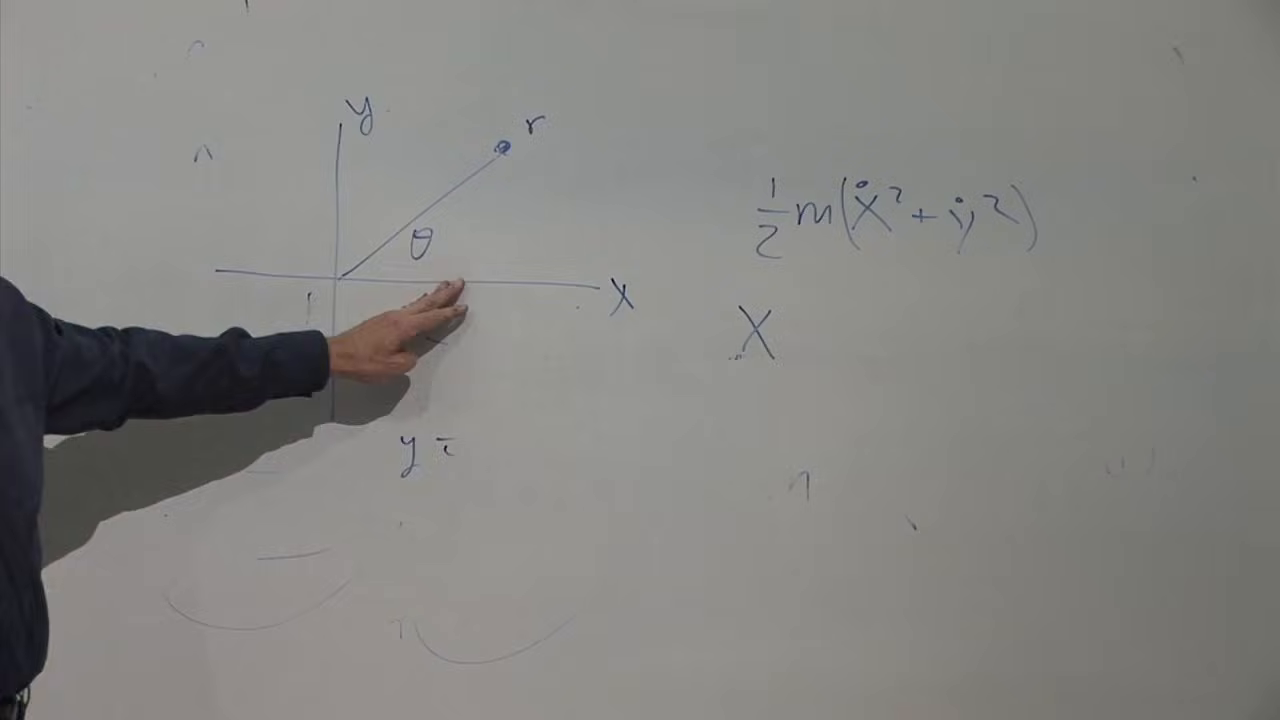
\includegraphics[width=0.80\textwidth]{lecture_03_figure_15.png}
  \caption{极坐标几何以及动能分解为径向运动和角向运动。}
  \lectureframe{01:23:30}
\end{figure}

径向方程为
\begin{equation}
  m\ddot r
  =mr\dot\theta^2-\frac{dV}{dr}.
  \label{eq:radial-equation}
\end{equation}
第一项是与粒子自身角向运动相关的向外离心贡献。

对于角度，
\begin{equation}
  \frac{d}{dt}\left(\frac{\partial L}{\partial\dot\theta}\right)
  =\frac{\partial L}{\partial\theta}=0,
  \label{eq:theta-el}
\end{equation}
因为中心势没有显式的 \(\theta\) 依赖。因此
\begin{equation}
  \frac{d}{dt}\left(mr^2\dot\theta\right)=0,
  \qquad
  mr^2\dot\theta=\ell,
  \label{eq:angular-momentum}
\end{equation}
其中 \(\ell\) 是守恒的角动量。

\begin{figure}[htbp]
  \centering
  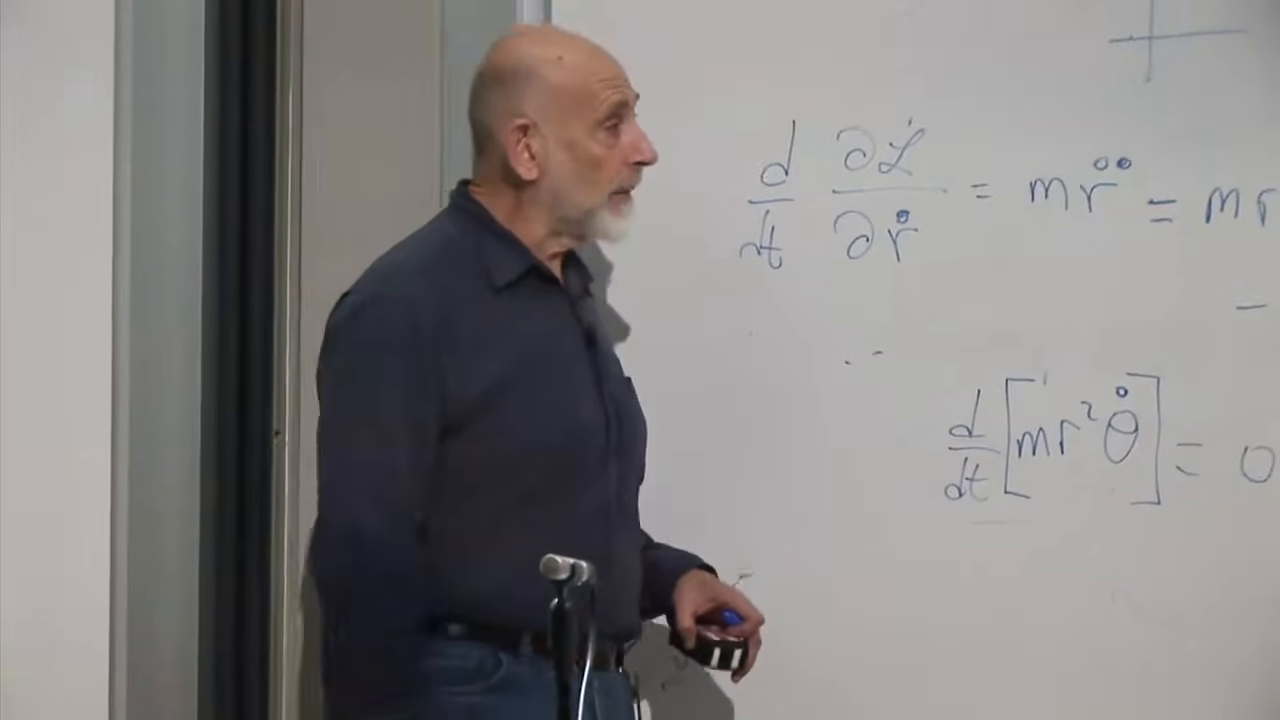
\includegraphics[width=0.82\textwidth]{lecture_03_figure_16.png}
  \caption{角向的欧拉--拉格朗日方程右端为零，
  从而揭示出 \(mr^2\dot\theta\) 的守恒。}
  \lectureframe{01:29:25}
\end{figure}

角向方程给出
\begin{equation}
  \dot\theta=\frac{\ell}{mr^2}.
  \label{eq:theta-dot-angular-momentum}
\end{equation}
代入式~\eqref{eq:radial-equation}后，只剩下关于
\(r\) 的一个方程：
\begin{equation}
  m\ddot r
  =\frac{\ell^2}{mr^3}-\frac{dV}{dr}.
  \label{eq:effective-radial-equation}
\end{equation}

在 \(L\) 中不出现的坐标，传统上称为\emph{循环}坐标，即使它不是角度也是如此。如果 \(q\) 是循环坐标，那么
\begin{equation}
  \frac{\partial L}{\partial q}=0
  \quad\Longrightarrow\quad
  \frac{d}{dt}\left(\frac{\partial L}{\partial\dot q}\right)=0.
  \label{eq:cyclic-conservation}
\end{equation}
其共轭动量守恒。这是对对称性与守恒定律之间一般联系的第一瞥。

\section{关于意义、能量与范围的问题}

接下来的问题揭示了这一形式体系的更深层内容所在。

\begin{classroomqa}
  \audiencequestion{除了发现拉格朗日量能给出正确的经典方程之外，是否还有独立的理由得到它？\lecturetimestamp{01:33:25--01:35:07}}
  \lecturerresponse{从历史上看，一个多世纪的经典力学表明，粒子、波和电磁场都可以写成这种形式。在经典层面上，这种累积的成功是关于定律如何组织起来的经验事实。更深层的解释来自量子力学，此处暂不讨论。}
\end{classroomqa}

\begin{classroomqa}
  \audiencequestion{在旋转参考系的拉格朗日量中，速度线性项能否被赋予普通的动能或势能？\lecturetimestamp{01:35:08--01:36:23}}
  \lecturerresponse{不能。与时间平移相关的守恒量是通过哈密顿量构造得到的，而不是通过把 \(L\) 中的每一项都读作动能或势能。对于式~\eqref{eq:rotating-lagrangian}，速度线性项在 \(\sum_a\dot q_a\,\partial L/\partial\dot q_a-L\) 中相消。哈密顿量处理将系统地组织这一点。}
\end{classroomqa}

确实，因为 \(L_{\mathrm{rot}}\) 没有显式的时间依赖，
\begin{equation}
  \begin{aligned}
    H_{\mathrm{rot}}
    &=\dot X\frac{\partial L}{\partial\dot X}
     +\dot Y\frac{\partial L}{\partial\dot Y}-L\\
    &=\frac{m}{2}(\dot X^2+\dot Y^2)
     -\frac{m\omega^2}{2}(X^2+Y^2)
  \end{aligned}
  \label{eq:rotating-hamiltonian-preview}
\end{equation}
是守恒的。它是旋转参考系中的雅可比积分，而不是惯性观察者所赋予的同一个数值能量。依赖于时间的坐标变换不必保持能量的数值形式。

\begin{classroomqa}
  \audiencequestion{如果弯曲轨迹是由引力引起的呢？\lecturetimestamp{01:36:30--01:37:10}}
  \lecturerresponse{对于牛顿引力，只需在中心力拉格朗日量中使用
  \(V(r)=-GMm/r\)。弯曲时空属于广义相对论，这里不作假设。}
\end{classroomqa}

\begin{classroomqa}
  \audiencequestion{离心势及其能量仅仅是虚构的吗？\lecturetimestamp{01:37:13--01:40:14}}
  \lecturerresponse{旋转平台上的观察者测量到有效力，并且可以一致地使用旋转参考系的守恒量。\emph{虚构}意味着这些项来自非惯性描述，而不是说它们观测到的效应是想象出来的。能量本身在一般的依赖于时间的坐标变换下并不不变。}
\end{classroomqa}

\begin{classroomqa}
  \audiencequestion{依赖于速度的科里奥利力指向什么方向？\lecturetimestamp{01:40:22--01:42:36}}
  \lecturerresponse{它垂直于旋转参考系中的速度，其大小与速率和参考系的角速度成正比。在平面内，各分量交换 \(\dot X\) 和 \(\dot Y\) 并带有相反的符号，如式~\eqref{eq:rotating-equations}所示。}
\end{classroomqa}

\begin{figure}[htbp]
  \centering
  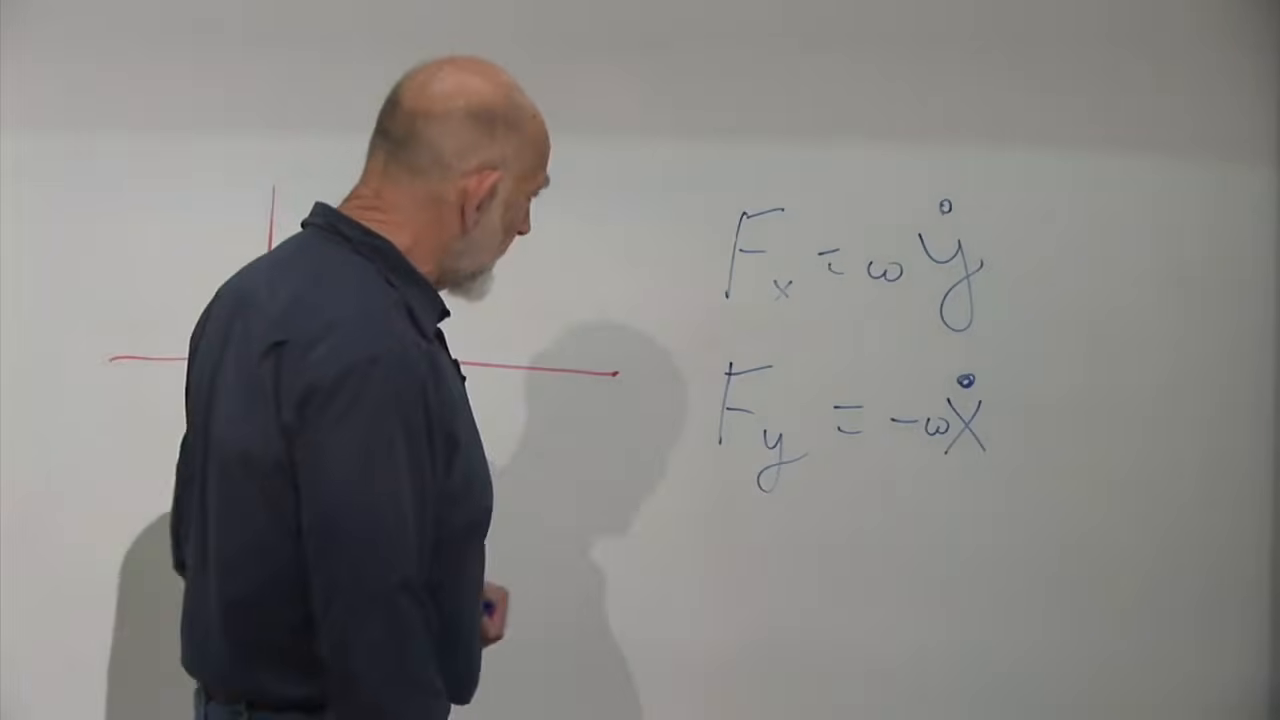
\includegraphics[width=0.76\textwidth]{lecture_03_figure_17.png}
  \caption{交叉速度分量模式：科里奥利力垂直于旋转参考系中的速度。}
  \lectureframe{01:41:40}
\end{figure}

\begin{classroomqa}
  \audiencequestion{起始拉格朗日量必须在惯性系中写出吗？\lecturetimestamp{01:42:37--01:44:00}}
  \lecturerresponse{对于普通的自由粒子，牛顿的惯性系定律给出了简单的起始形式 \(m(\dot x^2+\dot y^2)/2\)。一旦知道了这一物理定律，作用量就可以变换到任何其他坐标。不应独立地假设在旋转参考系中也有同样的简单动能公式。}
\end{classroomqa}

同一种速度线性项也出现在磁场中的带电粒子情形：
\begin{equation}
  L_{\mathrm{em}}
  =\frac12m\mathbf v^2
   +q\mathbf A(\mathbf r,t)\cdot\mathbf v
   -q\phi(\mathbf r,t).
  \label{eq:electromagnetic-lagrangian}
\end{equation}
对于垂直于平面的均匀磁场，对称规范 \(\mathbf A=\tfrac12\mathbf B\times\mathbf r\) 产生一个正比于
\(X\dot Y-Y\dot X\) 的项，其代数结构与科里奥利项相同。

\begin{figure}[htbp]
  \centering
  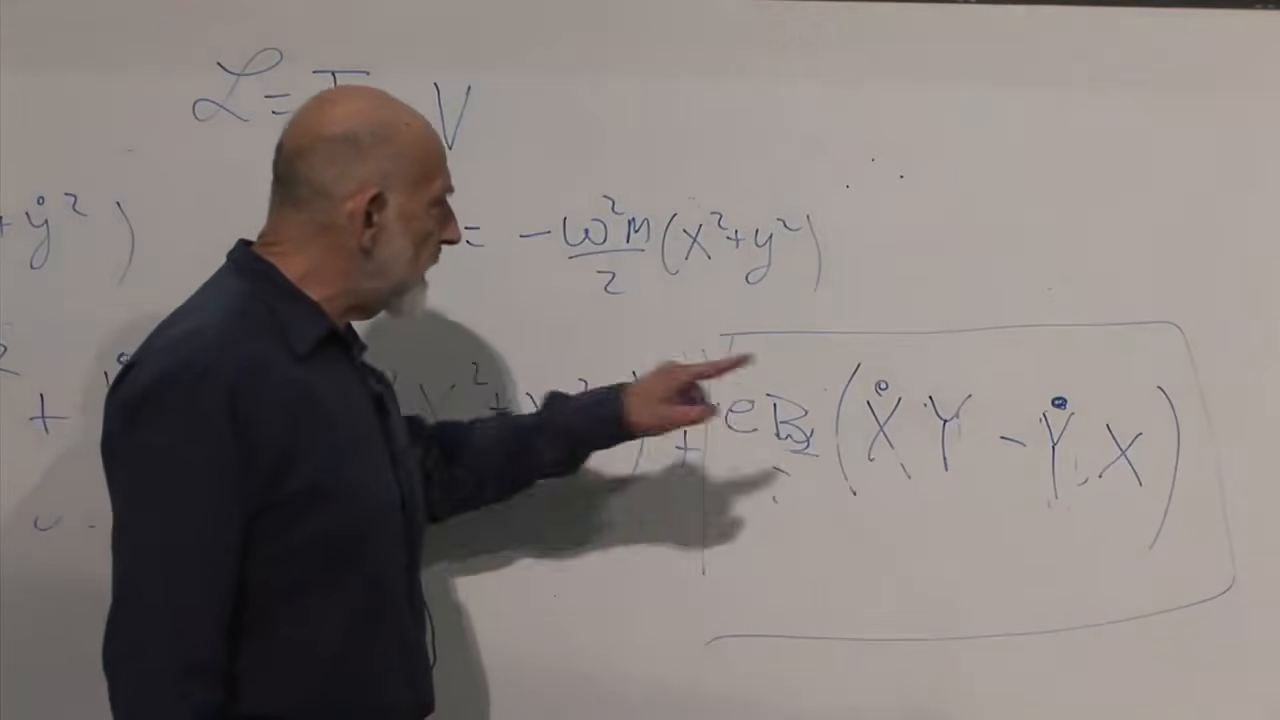
\includegraphics[width=0.82\textwidth]{lecture_03_figure_18.png}
  \caption{这个速度线性旋转坐标系项，正是促使人们将其与均匀磁场中的带电粒子进行比较的原因。}
  \lectureframe{01:44:40}
\end{figure}

\begin{classroomqa}
  \audiencequestion{对于什么函数可以充当拉格朗日量，除了光滑性之外，是否还有约束？\lecturetimestamp{01:44:46--01:45:06}}
  \lecturerresponse{有，但相关的约束需要比目前已经展开的更多的结构，因此推迟讨论。在现阶段，核心的教益是一个提出的拉格朗日量如何生成方程和守恒定律。}
\end{classroomqa}

旋转方程也允许圆周运动：在惯性系中固定的一个点，从旋转木马上看，会绕旋转原点做圆周运动。磁类比于是解释了为什么带电粒子能够执行回旋圆周运动。

\begin{classroomqa}
  \audiencequestion{带电粒子会停留在那个圆上，还是辐射会使轨道坍缩？\lecturetimestamp{01:46:11--01:47:21}}
  \lecturerresponse{正在讨论的仅涉及粒子的方程忽略了辐射。一旦把与电磁场的耦合以及辐射反作用包括进来，加速的经典电荷就可以辐射。因此，辐射是进一步的物理效应，而不是对截断方程中轨道的矛盾。}
\end{classroomqa}

\begin{classroomqa}
  \audiencequestion{飓风与这个讨论有什么关系？
  \lecturetimestamp{01:47:30--01:47:50}}
  \lecturerresponse{它们的大尺度大气运动发生在旋转的地球上，因此科里奥利效应很重要。恰当的推导属于气象学，这里不尝试进行。}
\end{classroomqa}

\begin{classroomqa}
  \audiencequestion{作用量框架是否被期望涵盖每一条物理定律，而一个真正的例外又意味着什么？\lecturetimestamp{01:47:57--01:49:01}}
  \lecturerresponse{在讨论范围内的每一个已知的封闭基础理论都可以用作用量来组织：牛顿粒子、麦克斯韦场、广义相对论以及标准模型。诸如黏性阻力之类的表面反例，是在环境自由度被省略时出现的。把系统扩大到包括流体或微观热浴，基础描述就再次符合该框架。因此，一个真正基础的例外将会是一项重大发现。}
\end{classroomqa}
